\section{Numerical Simulations}
\begin{frame}{Example: One-Dimensional Shear Flow}
	\scriptsize
Consider
	\begin{align}
		\partial_t Q(x,t) + \textcolor{blue}{A}\partial_x Q(x,t) = \textcolor{red}{\varphi} (Q(x,t)), \label{conservationlaws}
	\end{align}
	where $Q(x,t) = (f_0, c^{-2}_2, c^{-1}_2, ..., c^2_2)$ is. \\
	\vspace{0.5cm}
	Solve this problem by splitting it into two subproblems of the form
	\begin{enumerate}
		\item $\partial_t Q(x,t)  = \varphi (Q(x,t))$
		\item $\partial_t Q(x,t) + A Q_x=0$.
	\end{enumerate}
\end{frame}

\begin{frame}
	\scriptsize
	\begin{enumerate}
		\item Solve the drift diffusion equation
		\begin{equation*}
			\partial_t \left(\begin{array}{c}
				f_0 \\
				c_2^{-2} \\
				c_2^{-1} \\
				c_2^0 \\
				c_2^1 \\
				c_2^2
			\end{array}\right)  = \begin{pmatrix}
				0 & 0 & 0 & 0 & 0 & 0 \\
				0 & -6D_r & \frac{2}{7}w_x & 0 & 0 & 0 \\
				-\frac{\sqrt{15}}{5}w_x & -\frac{5}{7}w_x & -6D_r & \frac{3\sqrt{3}}{7}w_x & 0 & 0 \\
				0 & 0 & -\frac{4\sqrt{3}}{7}w_x & -6D_r & 0 & 0 \\
				0 & 0 & 0 & 0 & -6D_r & -\frac{5}{7} w_x\\
				0 & 0 & 0 & 0 & \frac{2}{7}w_x & -6D_r
			\end{pmatrix} \cdot
			\left(\begin{array}{c}
				0 \\
				c^{-2}_2(t) \\
				c_2^{-1}(t) \\
				c_2^0(t) \\
				c_2^1(t) \\
				c_2^2(t)
			\end{array}\right).
		\end{equation*}
		with Runge-Kutta 4th order method .
		\item Solve the advection equation
		$$
		\partial_t \left(\begin{array}{c}
			f_0 \\
			c_2^{-2} \\
			c_2^{-1} \\
			c_2^0 \\
			c_2^1 \\
			c_2^2
		\end{array}\right) + \begin{pmatrix}
			0 & 0 & \frac{\sqrt{15}}{15} & 0 & 0 & 0 \\
			0 & 0 & \frac{1}{7} & 0 & 0 & 0 \\
			\frac{\sqrt{15}}{15} & \frac{1}{7} & 0 & \frac{\sqrt{3}}{21} & 0 &  0 \\
			0 & 0 & \frac{\sqrt{3}}{21} & 0 & 0 & 0 \\
			0 & 0 & 0 & 0 & 0 & \frac{1}{7}\\
			0 & 0 & 0 & 0 & \frac{1}{7} & 0
		\end{pmatrix} \partial_x \left(\begin{array}{c}
			f_0 \\
			c_2^{-2} \\
			c_2^{-1} \\
			c_2^0 \\
			c_2^1 \\
			c_2^2
		\end{array}\right) = 0
		$$
		with one-dimensional resolution Wave Propagation Algorithm.
	\end{enumerate}
\end{frame}

\begin{frame}{Macroscopic Transport}
	\scriptsize
	Consider a Riemann Problem for externally imposed shear flow with $wx/D_r = 0.5$ for the left state and $wx/D_r = 1$ for the right state.
	\begin{figure}[H]
		\centering
		\begin{minipage}{0.32\textwidth}
			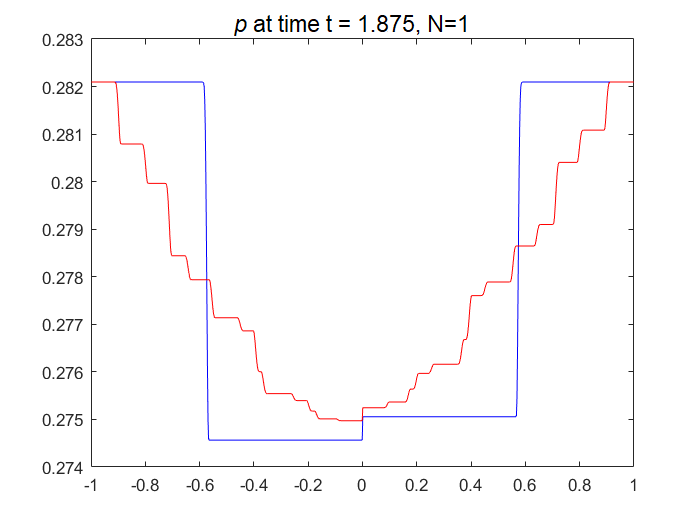
\includegraphics[width=\textwidth]{Bilder_wx/Wavepropa/red=12th_blue=2nd_wx=1_leftDr1_rightDr2_Awp12th}
		\end{minipage}
		\hfill
		\begin{minipage}{0.32\textwidth}
			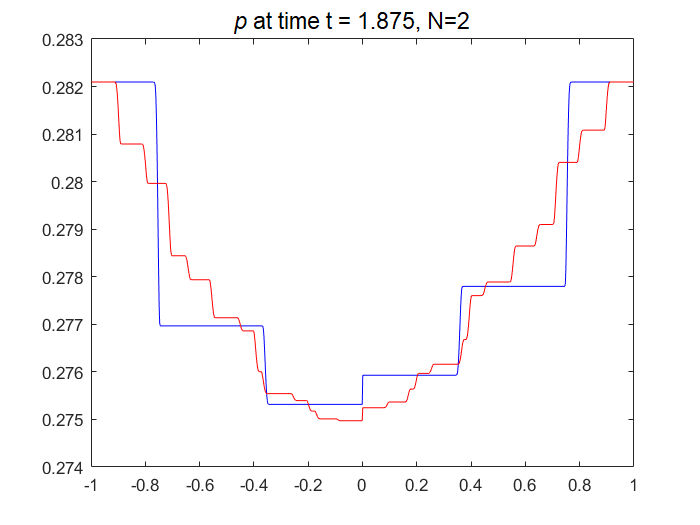
\includegraphics[width=\textwidth]{Bilder_wx/Wavepropa/red=12th_blue=4th_wx=1_leftDr1_rightDr2_Awp12th}
		\end{minipage}
		\hfill
		\begin{minipage}{0.32\textwidth}
			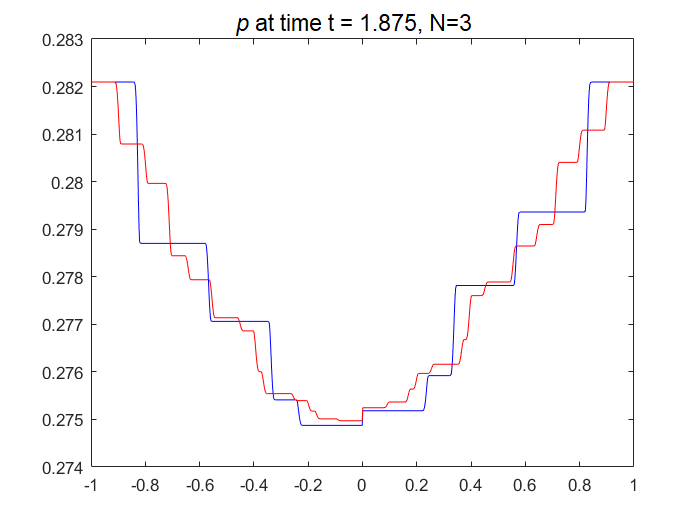
\includegraphics[width=\textwidth]{Bilder_wx/Wavepropa/red=12th_blue=6th_wx=1_leftDr1_rightDr2_Awp12th}
		\end{minipage}
		\vfill
		\begin{minipage}{0.32\textwidth}
			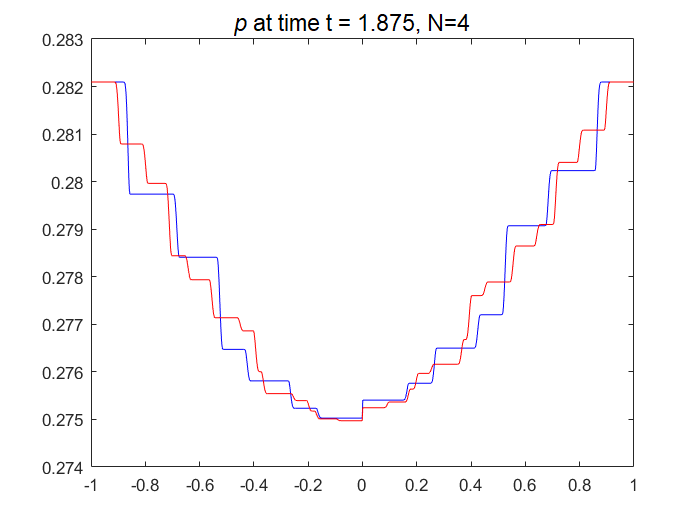
\includegraphics[width=\textwidth]{Bilder_wx/Wavepropa/red=12th_blue=8th_wx=1_leftDr1_rightDr2_Awp12th}
		\end{minipage}
		\hfill
		\begin{minipage}{0.32\textwidth}
			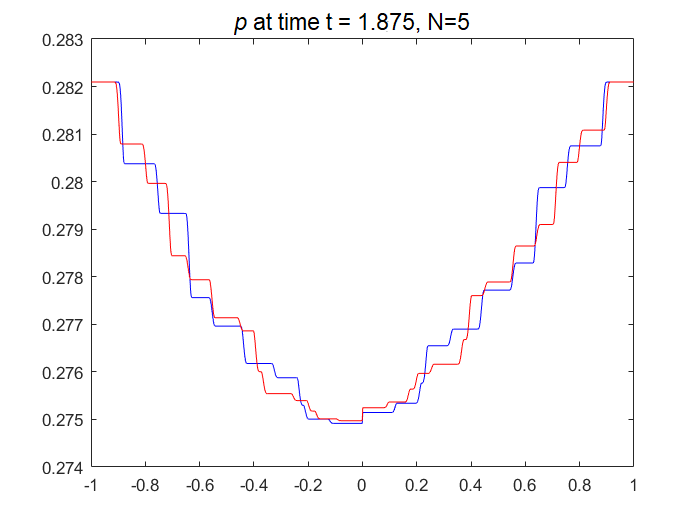
\includegraphics[width=\textwidth]{Bilder_wx/Wavepropa/red=12th_blue=10th_wx=1_leftDr1_rightDr2_Awp12th}
		\end{minipage}
		\hfill
		\begin{minipage}{0.3\textwidth}
			% Optional: Leave empty or add another image
		\end{minipage}
		\caption{Solution of the Riemann problem for $f_0$ at the time $t = 1.875$ using the moment system for different $N$ (blue curve) in comparison with $N = 6$ (red curve).}
	\end{figure}
\end{frame}

\begin{frame}
	\scriptsize
	\textbf{Setting:}\\
	\begin{itemize}
		\item $w_{xi} = \pi \cdot \cos(\pi\cdot x_i)$
		\item Initial value $q(i,1)$ is set to $\frac{1}{2\sqrt{\pi}}$, rest $0$
		\item grid cells in x direction is set to $1000$
	\end{itemize}
	\begin{figure}[H]
		\centering
		\begin{minipage}{0.32\textwidth}
			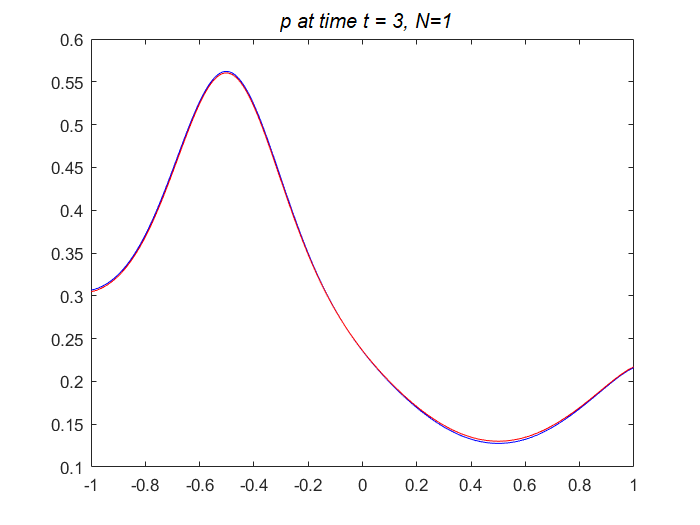
\includegraphics[width=\textwidth]{Bilder_wx/Wavepropa/red=12th_blue=2nd_wx=sin(pix)_Awp=0.5sqrt(pi)}
		\end{minipage}
		\hfill
		\begin{minipage}{0.32\textwidth}
			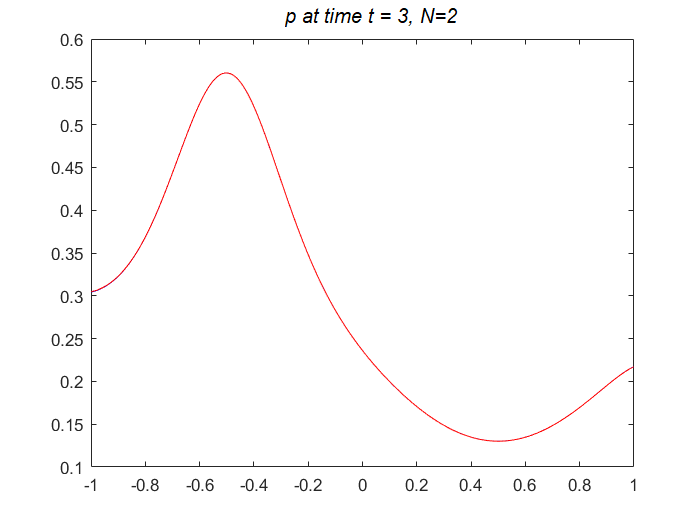
\includegraphics[width=\textwidth]{Bilder_wx/Wavepropa/red=12th_blue=4th_wx=sin(pix)_Awp=0.5sqrt(pi)}
		\end{minipage}
		\hfill
		\begin{minipage}{0.32\textwidth}
			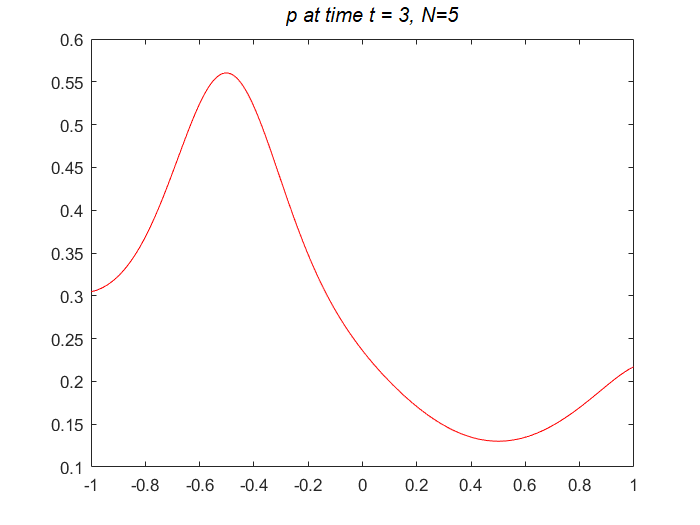
\includegraphics[width=\textwidth]{Bilder_wx/Wavepropa/red=12th_blue=10th_wx=sin(pix)_Awp=0.5sqrt(pi)}
		\end{minipage}
		\caption{Solution of the problem (\ref{conservationlaws}) for $f_0$ at the time $t = 3$ using the moment system for different $N$ (blue curve) in comparison with $N = 6$ (red curve).}
	\end{figure}
\end{frame}

\begin{frame}{Simulation of One-Dimensional Coupled Shear Flow Problem}
\scriptsize
Consider the coupled moment system
\begin{align*}
&\partial_t Q(\boldsymbol{x},t) + A\partial_x Q(\boldsymbol{x},t) =\varphi (Q(\boldsymbol{x},t)) \\
	&Re\partial_{x}w = \partial_{xx}w + \delta(\bar{\rho}-\rho(x,t)).
\end{align*}
on the interval $[0, 100]$ with periodic boundary conditions and initial data
\begin{align*}
	&\rho(x,0) = exp(-10(x-50)^2), \\
	&w(x,0) = 1 ,\\
	&D_r = 0.01, \delta = 1
\end{align*}
\end{frame}